\chapter{Ispitni skupovi izvornih slika}

Za treniranje naših modela koristili smo skupove podataka CIFAR-10 [\cite{alexkrizhevsky2009}] i MNIST.\\
CIFAR-10 (Canadian Institute For Advanced Research) je skup 60000 slika 32px$\times$32px u boji te ima 10 klasa sa 6000 slika po klasi.

\begin{figure}[h]
	\centering{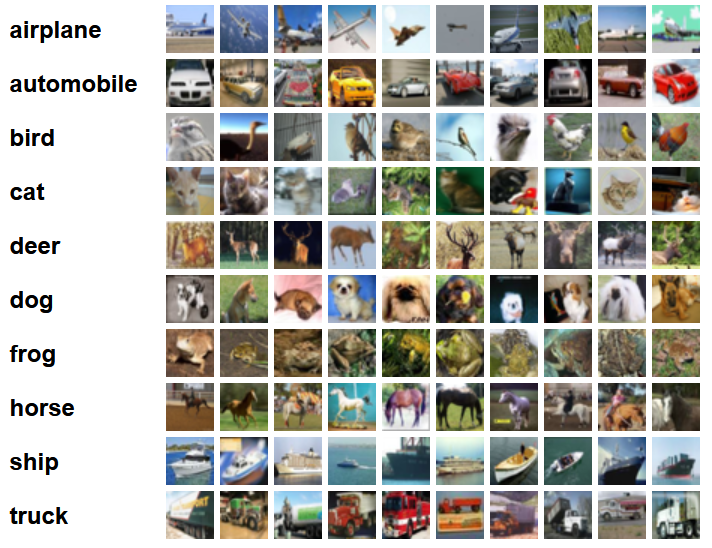
\includegraphics[scale=0.75]{slike/cifar10.png}}
	\caption{Nasumične slike iz 10 klasa skupa CIFAR}
	\label{cifar}
\end{figure}

Klase su međusobno isključive te ne postoji presjek između npr. kamiona i automobila. \pagebreak

MNIST (Modified National Institute of Standards and Technology) je skup 70000 malih slika, 28px$\times$28px ručno napisanih brojeva. Naravno ima 10 ravnomjerno raspoređenih klasa, znamenke od 0 do 9.\\

\begin{figure}[h]
	\centering{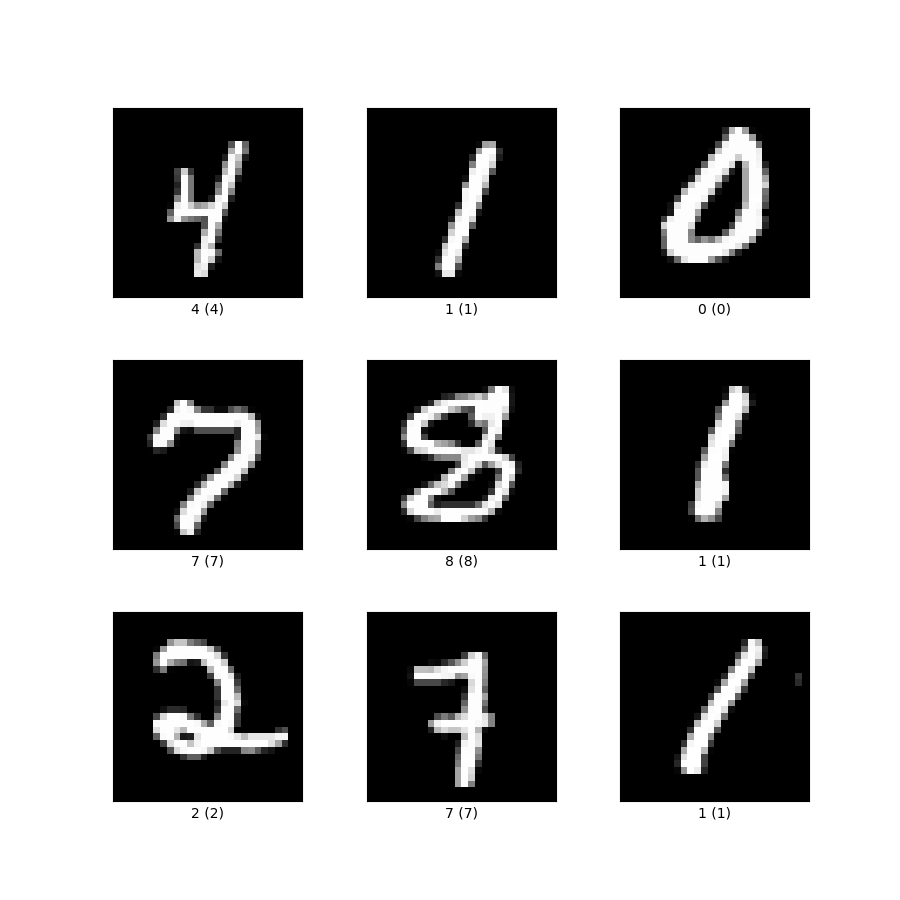
\includegraphics[scale=0.5]{slike/mnist.png}}
	\caption{Nasumične slike iz skupa MNIST}
	\label{mnist}
\end{figure}